\documentclass{beamer}
\usepackage{latexsym}
\usepackage{graphicx}
\usetheme{Warsaw}

\title{Chapter 1}
\subtitle{ML Introduction}

\begin{document}
\maketitle

\begin{frame}
  \frametitle{Math/stats background}
  \begin{itemize}
  \item Partial derivatives, e.g.: \\
    \[
    \frac{\partial (x^3 + y^2 + 1)}{\partial x}
    \]
  \item Matrix and vector operations \\
    \[
    \begin{bmatrix}
      1 & 2  & 3\\
      4 & 5  & 6
    \end{bmatrix} \times  \begin{bmatrix}
      7 \\
      8 \\
      9
    \end{bmatrix} =  \begin{bmatrix}
      1 \times 7 + 2 \times 8 + 3 \times 9 \\
      4 \times 7 + 5 \times 8 + 6 \times 9
    \end{bmatrix} = \begin{bmatrix}
      50 \\
      122
    \end{bmatrix}
    \]
  \item Basic probability and statistics
    \begin{itemize}
    \item Conditional probability
    \item Normal distribution
    \end{itemize}
  \end{itemize}
\end{frame}

\begin{frame}
  \frametitle{Programming background}
  \begin{itemize}
  \item Python
  \item NumPy
  \item Matplotlib
  \end{itemize}
\end{frame}

\begin{frame}
  \frametitle{What is ML? Ask Wikipedia}
  \begin{quote}
    Machine learning is a subfield of computer science (more particularly soft computing) that evolved from the study of pattern recognition and computational learning theory in artificial intelligence. In 1959, Arthur Samuel defined machine learning as a "Field of study that gives computers the ability to learn without being explicitly programmed". Machine learning explores the study and construction of algorithms that can learn from and make predictions on data.
  \end{quote}
  \href{http://machinelearningmastery.com/what-is-machine-learning/}{More definitions here}
\end{frame}

\begin{frame}
  \frametitle{Applications of ML}
  \begin{itemize}
  \item Image recognition
  \item Spam classification
  \item Web search engines
  \item Voice recognition
  \item \href{https://www.quora.com/What-are-some-real-world-examples-of-applications-of-machine-learning-in-the-field}{Link to Quora}
  \end{itemize}
\end{frame}

\begin{frame}
  \frametitle{Three types of ML}
  \begin{itemize}
  \item Supervised learning
  \item Unsupervised learning
  \item Reinforcement learning
  \end{itemize}
\end{frame}

\begin{frame}
  \frametitle{Yann LeCun explains supervised learning}
  \scriptsize
  A pattern recognition system is like a black box with a camera at one end, a green light and a red light on top, and a whole bunch of knobs on the front. The learning algorithm tries to adjust the knobs so that when, say, a dog is in front of the camera, the red light turns on, and when a car is put in front of the camera, the green light turns on. You show a dog to the machine. If the red light is bright, don't do anything. If it’s dim, tweak the knobs so that the light gets brighter. If the green light turns on, tweak the knobs so that it gets dimmer. Then show a car, and tweak the knobs so that the red light get dimmer and the green light gets brighter. If you show many examples of the cars and dogs, and you keep adjusting the knobs just a little bit each time, eventually the machine will get the right answer every time.
  \center
  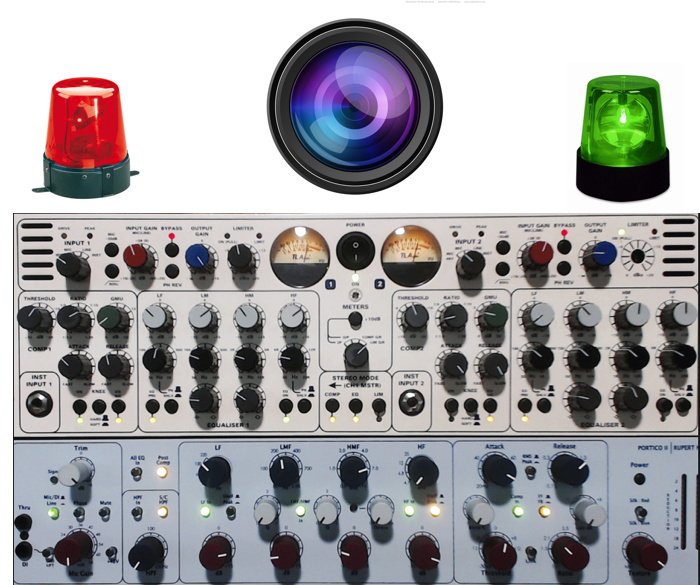
\includegraphics[scale=0.3]{Images/knobs.png}
\end{frame}

\begin{frame}
  \frametitle{Scaling up}
  The interesting thing is that it may also correctly classify cars and dogs it has never seen before. The trick is to figure out in which direction to tweak each knob and by how much without actually fiddling with them. This involves computing a “gradient,” which for each knob indicates how the light changes when the knob is tweaked.
  \\~\\
  Now, imagine a box with 500 million knobs, 1,000 light bulbs, and 10 million images to train it with. That’s what a typical Deep Learning system is.
  \\~\\
  Source: \href{http://spectrum.ieee.org/automaton/robotics/artificial-intelligence/facebook-ai-director-yann-lecun-on-deep-learning}{IEEE Spectrum Interview}
\end{frame}

\begin{frame}
  \frametitle{Supervised learning}
  \includegraphics[width=\textwidth]{Code/ch01/images/01_02.png}
  \begin{itemize}
  \item Predicting the future with supervised learning
  \item Classification vs. Regression
  \end{itemize}
\end{frame}

\begin{frame}
  \frametitle{Classification}
  \begin{columns}[c]
    \column{0.5\textwidth}
    \begin{itemize}
    \item Predict categorical class labels based on past observations
    \item Class labels are discrete unordered values
    \item Email spam classification example (binary)
    \item Handwritten digit classification example (multi-class)
    \end{itemize}
    \column{0.5\textwidth}
    \includegraphics[width=\textwidth]{Code/ch01/images/01_03.png}
  \end{columns}
\end{frame}

\begin{frame}
  \frametitle{Regression}
  \begin{itemize}
  \item Also a kind of supervised learning
  \item Prediction of continuous outcomes
  \item Predicting semester grades scores for students
  \end{itemize}
  \center
  \includegraphics[scale=0.4]{Code/ch01/images/01_04.png}
\end{frame}

\begin{frame}
  \frametitle{Unsupervised learning}
  \begin{itemize}
  \item Dealing with \textit{unlabeled} data
  \item Cluster analysis
  \item Objects within a cluster share a degree of similarity
  \end{itemize}
  \center
  \includegraphics[scale=0.4]{Code/ch01/images/01_06.png}
\end{frame}

\begin{frame}
  \frametitle{Unsupervised learing example}
  \begin{itemize}
  \item Latent Dirichlet Allocation (LDA)
  \item \href{http://www.princeton.edu/~achaney/tmve/wiki100k/browse/topic-presence.html}{Link to Wikipedia topics}
  \item \href {https://en.wikipedia.org/wiki/Latent_Dirichlet_allocation}{Wikipedia LDA entry}
    \item \href{http://blog.echen.me/2011/06/27/topic-modeling-the-sarah-palin-emails/}{Sara Palin topics}
  \end{itemize}
\end{frame}

\begin{frame}
  \frametitle{Iris dataset}
  \includegraphics[scale=0.1]{Code/ch01/images/01_08.png}
\end{frame}

\begin{frame}
  \frametitle{Basic terminology}
  \begin{itemize}
  \item Measurements of 150 iris flowers (150 samples / 4 features)
  \item From 3 different species (Setosa, Versicolor, Virginica)
  \item Rows are samples and columns are features
  \item $150 \times 4$ matrix $\mathbf{X} \in \mathbb{R}^{150 \times 4}:$
  \end{itemize}

  \[
  \begin{bmatrix}
    x_{1}^{(1)} & x_{2}^{(1)} & x_{3}^{(1)} & \dots  & x_{4}^{(1)} \\
    x_{1}^{(2)} & x_{2}^{(2)} & x_{3}^{(2)} & \dots  & x_{4}^{(2)} \\
    \vdots & \vdots & \vdots & \ddots & \vdots \\
    x_{1}^{(150)} & x_{2}^{(150)} & x_{3}^{(150)} & \dots  & x_{4}^{(150)}
  \end{bmatrix}
  \]
\end{frame}

\begin{frame}
  \frametitle{A roadmap for building ML systems}
  \includegraphics[width=\textwidth]{Code/ch01/images/01_09.png}
\end{frame}

\begin{frame}
  \frametitle{Model selection}
  \begin{itemize}
  \item No Free Lunch Theorems
  \item Each classification algorithm makes assumptions
  \item Often we empirically determine what works best
  \item But how do we know what works best?
    \begin{itemize}
    \item Classification accuracy
    \item Train+Dev+Test split
    \item Hyperparameter optimization (knobs of the model)
    \end{itemize}
  \end{itemize}
\end{frame}

\begin{frame}
  \frametitle{Python for ML}
  \begin{itemize}
  \item Libraries for scientific computing such as NumPy and SciPy
  \item Performance of interpreted languages is inferior
  \item But NumPy and SciPy build upon lower level C and Fortran subroutines
  \item Scikit-learn library
  \item See page 13 for installation instructions (or just google)
  \item \href{http://www-ekp.physik.uni-karlsruhe.de/~giffels/GridKa-School-Lectures/NumPy.slides.html}{\beamerbutton{NumPy Slides}}
  \end{itemize}
\end{frame}

\end{document}
